
%% ==================================================================================================
%%
\documentclass[12pt]{book}
\usepackage{amsfonts}
\usepackage{amsmath}
\usepackage{amssymb}
\usepackage{graphicx}
\usepackage{hyperref}
\usepackage{float}
\usepackage{verbatim}
\usepackage{xlop} %% for multiplication https://tex.stackexchange.com/questions/11702/how-to-present-a-vertical-multiplication-addition
\usepackage{listings} %% to format generic computer code
\usepackage{lmodern} % for bold teletype font
\usepackage{minted} % colour Java code

\usepackage{tasks}
%\NewTasks[style=enumerate,counter-format=tsk[A].,label-width=3ex]{choice}[\item](4)

%% =======   set page margins    =======
\setlength{\textheight}{10in}
\setlength{\textwidth}{7.4in}
\setlength{\topmargin}{-0.75in}
\setlength{\oddsidemargin}{-0.5in}
\setlength{\evensidemargin}{-0.5in}
\setlength{\parskip}{0.15in}
\setlength{\parindent}{0in}

%%  for European long division
% https://tex.stackexchange.com/questions/432435/how-to-set-up-european-french-style-long-division-in-tex
\newcommand\frdiv[5]{%
    \[
    \renewcommand\arraystretch{1.5}
    \begin{array}{l| l}
    #1 & #2 \\
    \cline{2-2}
    #3 & #4 \\
    \cline{1-1}
    #5 & \\
    \end{array}
    \]
}

%%  for European long division


%% ==================================================================================================

\begin{document}

\newcommand{\reporttitle}{Assignment 1}
\newcommand{\reportauthorOne}{Kien Do}
\newcommand{\cidOne}{300163370}
\input{titlePage/titlepage.txt}



%% ==================================================================================================

%%%%%%%%%%%% PROBLEMS START HERE

\begin{enumerate}
    %% ============================   New Item   ============================
    \item \textbf{Answer}
    
    Case 1: We draw white first, black second.
    \begin{align*}
        D_1 &= \dfrac{7}{7+5} \times \dfrac{5}{7+5} \\
        D_1 &= \dfrac{7}{13} \times \dfrac{5}{13} \\
        D_1 &= \dfrac{35}{132}
    \end{align*}
    Case 2: We draw black first, white second.
    \begin{align*}
        D_2 &= \dfrac{5}{7+5} \times \dfrac{7}{7+5} \\
        D_2 &= \dfrac{5}{13} \times \dfrac{7}{13} \\
        D_2 &= \dfrac{35}{132}
    \end{align*}
    Since both cases are true, one white ball is drawn and one black ball is drawn, regardless of the order, we simply add the probability of both cases together.
    \begin{align*}
        D &= \dfrac{35}{132} + \dfrac{35}{132} \\
        D &= \dfrac{70}{132} \\
        D &= \dfrac{35}{66}
    \end{align*}
    Therefore, the probability is $\dfrac{35}{66}$.
    
    %% ============================   New Item   ============================
    \item \textbf{Answer}
    \begin{enumerate}
        \item Another way to ask this question is how many permutations of rankings are possible. The first position has 7 possibilities (as there are 7 people). The second position has 6 possibilities (as there are 6 people left). The third position has 5 possibilities (as there are 5 people left), and so on. We have,
        $$7 \times 6 \times 5 \times 4 \times 3 \times 2 \times 1 = 5040$$
        As such, there are 5040 different possible rankings.
        
        \item The probability of a woman getting 1st place is $\frac{4}{7}$. The probability of a woman getting 2nd place is $\frac{3}{6}$. The probability of a woman getting 3rd place is $\frac{2}{5}$.The probability of a woman getting 4th place is $\frac{1}{4}$.\\
        By the multiplication rule, therefore probability of all women receiving the top 4 scores is
        $$\dfrac{4}{7} \times \dfrac{3}{6} \times \dfrac{2}{5} \times \dfrac{1}{4} = \dfrac{1}{35}$$
        
        \item The probability of a woman getting 1st place is $\frac{4}{7}$. The probability of a woman getting 2nd place is $\frac{3}{6}$. 
        By the multiplication rule, therefore probability of women receiving the top 2 scores is
        $$\dfrac{4}{7} \times \dfrac{3}{6} = \dfrac{2}{7}$$
    \end{enumerate}
    %% ============================   New Item   ============================
    \item \textbf{Answer}
    
    Start by writing down everything we know. Let,\\
    $P(K) = p$ \hfill be the probability that she knows the answer, \\
    $P(G) = 1-p$ \hfill be the probability that she guesses the answer,\\
    $P(R)$ \hfill be the probability that she gets the right answer,\\
    $P(R\,|\,G)=\frac{1}{n}$ \hfill be the probability that she gets the right answer, given that she guesses it,\\
    $P(R\,|\,K)=1$ \hfill be the probability that she gets the right answer, given that she knows it.
    
    Determine $P(K|R)$, the probability that she knows the answer given that she gets it right.\\
    
    By definition, we have that $P(K|R) = \dfrac{P(K \cap R)}{P(R)}$. Before computing $P(K|R)$, let's look at $P(R|K)$.
    \begin{align*}
        P(R|K) &= \dfrac{P(R \cap K)}{P(K)}\\
        P(R|K) &= \dfrac{P(K \cap R)}{P(K)}\\
        P(K \cap R) &= P(R|K) \times P(K)\\
        P(K \cap R) &= 1 \times p \qquad \xleftarrow[]{\text{substitute given values}}\\
        P(K \cap R) &= p
    \end{align*}
    So, by substitution, we have,
    $$P(K|R) = \dfrac{P(K \cap R)}{P(R)} = \dfrac{p}{P(R)}$$
    We do not have $P(R)$. But since it is an unconditional probability, we have that,
    \begin{align*}
        P(R) &= P(R|K) \times P(K) + P(R|K') \times P(K')\\
        P(R) &= P(R|K) \times P(K) + P(R|G) \times P(G) \quad \xleftarrow[]{P(K') = P(G)}\\
        P(R) &= (1)(p) + \left(\dfrac{1}{n}\right)(1-p)\\
        P(R) &= p + \left(\dfrac{1}{n}\right)(1-p)
    \end{align*}
    By substitution, we have that,
    \begingroup
    \addtolength{\jot}{1em}
    \begin{align*}
        P(K|R) = \dfrac{p}{P(R)} &= \dfrac{p}{p + \left(\frac{1}{n}\right)(1-p)}\\
        &= \dfrac{np}{np + (1-p)}\\
        &= \dfrac{np}{(n-1)p + 1}
    \end{align*}
    \endgroup
    Therefore, $$P(K|R) = \dfrac{np}{(n-1)p + 1}$$
    \newpage

    %% ============================   New Item   ============================
    \item \textbf{Answer}
    
    We know that in $60\%$ of all solar-heat installations, the utility bill is reduced by at least one-third. This is the same as saying one solar-heat installation has a probability of reducing the utility bill by one-third. 
    \begin{enumerate}
        \item We need to find out the probability of the utility bill being reduced by one-third if there are four out of five installations.
        
        First, we need to find out how many ways we can choose 4 installations out of 5. In other words,
        $${}_{5} C_{4} = 5$$
        
        Since each installation has a $60\%$ probability of reducing the utility bill, to find the probability of four installations having a probability of reducing the utility by one-third, we simply multiply the probability of one installation reducing the utility bill by the number of installations,
        $$(0.60)^4$$
        
        Similarly, since each non-installation has $40\%$ probability of NOT reducing the utility bill, to find the probability of one installation having a probability of NOT reducing the utility bill, we simply multiply the probability of one installation NOT reducing the utility bill by the number of non-installations,
        $$(0.40)^1$$
        
        To obtain the answer, we multiply all three results together,
        \begin{align*}
            &= {}_{5} C_{4} \times (0.60)^4 \times (0.40)^1 \\
            &= 5 \times (0.60)^4 \times (0.40)^1 \\
            &= 0.2592
        \end{align*}
        Therefore, the probability of 4 out of 5 installations reducing the utility bill by one-third is $25.92\%$.
        
        \item To find the probability that the utility bill is reduced by one-third for at least four of five installations, we simply need to find the probability that the bill will reduce for four installations plus the probability that the bill will reduce for five installations.
        
        We have already determined that the probability that the utility bill will reduce for four of five installations is 0.2592 from part a). To find the probability that the bill will reduce for five out five installations we would apply the same formula,
        \begin{align*}
            &= {}_{5} C_{5} \times (0.60)^5 \times (0.40)^0 \\
            &= 1 \times (0.60)^5 \times 1 \\
            &= 0.07776
        \end{align*}
        We then add both results together,
        $$\text{P(4/5 installations) + P(5/5 installations)}$$
        $$0.2592 + 0.0.07776 = 0.33696$$
        
        Therefore, the probability of at least 4 out of 5 installations reducing the utility bill by one-third is $33.696\%$.
        
        
        
    \end{enumerate}
    
    %% ============================   New Item   ============================
    
    \item \textbf{Answer}
    
    We know that $10\%$ of hard drives require repairs within the first year. This is equivalent to saying that a hard drive has a $10\%$ chance of requiring a repair within the first year, and consequently, a hard drive has a $90\%$ of NOT requiring a repair within the first year. We need to find out the probability of AT LEAST 5 hard drives failing if the research team buys 20.
    
    We can use the following formula to calculate the probability that a certain number of hard drives will fail out of the total number of hard drives.
    $$x\text{ drives fail} = {}_{\text{total drives}} C_{x} \times (0.1)^x \times (0.9)^{\text{total drives} - x}$$
    
    But since that formula only calculates the probability of failure for $x$ number of hard drives and we are looking for AT LEAST $x$ number of hard drives failing, we can simply compute the solution by using the summation of all the successes from 5 to 20 using that formula. 
    
    However, to reduce our computational time, we can compute the summation of failure (from 0 to 4, inclusive) and subtract that result from the probability that everything can happen, 1.
    
    So, we have,
    \begin{align*}
        &= 1 - \sum_{i=0}^{4} \left({}_{20}C_{i}\right)(0.1)^i(0.9)^{20-i}\\
        &= 0.04317
    \end{align*}
    Therefore, the probability that the research team will see AT LEAST 5 out of the 20 drives requiring repairs within the first year is $0.04317$ or $4.317\%$.
    
    % We know that $10\%$ of hard drives require repairs within the first year. This is equivalent to saying that a hard drive has a $10\%$ chance of requiring a repair within the first year. We need to find out the probability of 5 hard drives failing if the research team buys 20.
    
    % Let $A_i$ be the event that the $i$th hard drive requires a repair within the first year. We have that the probability of 5 out of 20 hard drives failing is the intersection of all the possible combinations that 4 out of 20 hard drives will fail,
    % $$P(A_1' \cap A_2' \cap A_3' \cap A_4' \cap A_5' \cap ... \cap A_{19} \cap A_20) + P(A_1' \cap A_2' \cap A_3' \cap A_4' \cap A_5 \cap A_6' \cap ... \cap A_{19} \cap A_{20}) + ...$$
    
    % We first need to find how many ways there are of choosing 5 hard drives that will fail out of all 20 hard drives, in order words, $${}_{20} C_{5} = 15504$$
    
    % Since each hard drive has a $10\%$ chance of requiring repairs and we are looking for the probability that 5 hard drives will require repairs, we can say that the probability of all 5 of the hard drives requiring repairs is $$(0.1)^5$$
    
    % Consequently, since each hard drive has a $90\%$ chance of NOT requiring repairs and we are looking for the probability that 15 hard drives will NOT require repairs, we can say that the probability of the remaining 15 of the hard drives NOT requiring repairs is $$(0.9)^{15}$$
    
    % To obtain our answer, the simply need to do the following,
    % \begin{align*}
    %     &= {}_{20} C_{5} \times (0.1)^5 \times (0.9)^{15} \\
    %     &= 15504 \times (0.1)^5 \times (0.9)^{15} \\
    %     &= 0.03192
    % \end{align*}
    
    % However, to compute 
    
    % Therefore, the probability of 5 out of 20 hard drives failing is $3.192\%$.
    
    \item \textbf{Answer}
    
    \begin{enumerate}
        \item Hypergeometric distribution (implies non-replacement, non-independent distribution). 
        
        We have 25 defective cars and $100 - 25 = 75$ non-defective cars. The company selects 10 cars, so the probability of 2 out of 10 cars being defective is,
        \begin{align*}
            P(D) &= \dfrac{{}_{25} C_{2} \times {}_{75} C_{8}}{{}_{100} C_{10}}\\
            P(D) &= 0.292387
        \end{align*}
        
        \item Binomial distribution (implies replacement, independent distribution).
        \begin{align*}
            P(D) &= {}_{10} C_{2} \times \left(\dfrac{25}{100}\right)^{2} \times \left(1 - \dfrac{25}{100}\right)^{8} \\
            P(D) &= 0.281567
        \end{align*}
    \end{enumerate}
    
    %% ============================   New Item   ============================
    \newpage
    \item \textbf{Answer}
    
    \begin{enumerate}
        \item Determine the value $a$.
        \begin{align*}
            1 &= \int_{0}^{1} a(x^3+1) \,dx \\
            1 &= a \left[\dfrac{1}{4}x^4 + x\right] \Big|_0^1 \\
            1 &= a \left(\dfrac{1}{4} + 1\right) \\
            a &= \dfrac{1}{\frac{1}{4} + 1} \\
            a &= \dfrac{4}{5} \\
            a &= 0.8
        \end{align*}
        
        \item Find the cumulative distribution function of $X$.
        
        Recall that the cumulative distribution function can be found by integrating the probability density function.
        $$F(x) = \int_{-\infty}^{x} f_x(t) \, dt$$
        \begin{align*}
            0 < x < 1 \, &: \, \int_{0}^{x} (0.8)(t^3+1) \, dt\\
            &= (0.8) \left[\dfrac{t^4}{4} + t\right] \Big|_{0}^{x}\\
            &= (0.8) \left(\dfrac{x^4}{4}+x\right)
        \end{align*}
        \begin{equation*}
            g(x)=
            \begin{cases}
                0 \quad &\text{if} \, x \leq 0 \\
                (0.8) \left(\dfrac{x^4}{4}+x\right) \quad &\text{if} \, 0 < x < 1 \\
                1 \quad &\text{if} \, x \geq 1 \\
            \end{cases}
        \end{equation*}
        
        \item Compute $E[X]$.
        
        Recall the definition of the mean of a continuous probability distribution function is,
        $$\mu = E[X] = \int_{-\infty}^{\infty} xf(x) \, dx$$
        But we are not integrating from $-\infty$ to $\infty$. So, for our case,
        \begin{align*}
            0 < x < 1 \, &: \, \int_{0}^{1} x (0.8) \left(x^3+1\right) \, dx\\
            \mu &= (0.8) \int_{0}^{1} x^4 + x \, dx \\
            \mu &= (0.8) \left(\dfrac{x^5}{5} + \dfrac{x^2}{2}\right) \Big|_{0}^{1}\\
            \mu &= (0.8) \left(\dfrac{1}{5} + \dfrac{1}{2}\right)\\
            \mu &= 0.56
        \end{align*}
        
        \item Compute $var[X]$.
        
        Recall the definition of the variance of a continuous probability distribution function is,
        $$\sigma^2 = E\left[(X-\mu)^2\right] = \int_{-\infty}^{\infty}(x-\mu)^2f(x) \, dx$$
        However, since we have found $\mu$ or $E[X]$, we can use the following relationship,
        $$E\left[(x-\mu)^2\right] = E(x^2) - \left[E(x)\right]^2$$
        We already know the value of $\left[E(x)\right]^2$, so we simply need to find $E(x^2)$ then find $E\left[(x-\mu)^2\right]$. Recall that
        $$E[X] = \int_{-\infty}^{\infty} xf(x) \, dx$$
        Therefore,
        $$E[X^2] = \int_{-\infty}^{\infty} x^2f(x) \, dx$$
        But we are not integrating from $-\infty$ to $\infty$. So, for our case,
        \begin{align*}
            0 < x < 1 \, : E[X^2] &= \int_{0}^{1} x^2f(x) \, dx\\
            E[X^2] &= \int_{0}^{1} x^2(0.8)(x^3+1) \, dx\\
            E[X^2] &= (0.8) \int_{0}^{1} x^5+x^2 \, dx\\
            E[X^2] &= (0.8) \left(\dfrac{x^6}{6}+\dfrac{x^3}{3}\right) \Big|_{0}^{1}\\
            E[X^2] &= (0.8) \left(\dfrac{1}{6}+\dfrac{1}{3}\right)\\
            E[X^2] &= 0.4
        \end{align*}
        Find the variance of this distribution by substituting values into $E\left[(x-\mu)^2\right] = E(x^2) - \left[E(x)\right]^2$
        \begin{align*}
            E\left[(x-\mu)^2\right] &= 0.4 - (0.56)^2\\
            E\left[(x-\mu)^2\right] &= 0.0864
        \end{align*}
    \end{enumerate}
    
    \newpage
    
    %% ============================   New Item   ============================
    
    \item \textbf{Answer}
    \begin{enumerate}
        \item Compute $E[W]$.
        \begin{align*}
            W &= rV^2\\
            E[W] &= E[rV^2]\\
            E[W] &= E[2 \times V^2]\\
            E[W] &= 2 \times E[V^2]
        \end{align*}
        Solve for $E[V^2]$.
        
        Recall the formulas, $\mathrm{Var}[X] = E[X^2] - E[X]^2$ and $SD[X] = \sqrt{\mathrm{Var}[X]}$.
        Rearrange the second formula, we have,
        \begin{align*}
            SD[X] &= \sqrt{\mathrm{Var}[X]} \\
            \mathrm{Var} &= SD[X]^2
        \end{align*}
        By substitution,
        \begin{align*}
            \mathrm{Var}[X] &= E[X^2] - E[X]^2 \\
            SD[X]^2 &= E[X^2] - E[X]^2 \\
            E[X^2] &= SD[X]^2 + E[X]^2
        \end{align*}
        Therefore, we have that,
        \begin{align*}
            E[W] &= 2 \times E[V^2] \\
            E[W] &= 2 \times \left(SD[V]^2 + E[V]^2\right)
        \end{align*}
        We were given SD[X] = 2 and E[X] = 6, so we can simply substitute these values into our formula and determine $E[W]$.
        \begin{align*}
            E[W] &= 2 \times \left((2)^2 + (6)^2\right) \\
            E[W] &= 2 \times \left(4 + 36\right) \\
            E[W] &= 80
        \end{align*}
        
        \item Compute P($W >$ 128).
        
        This is my illustration of the problem.
        
        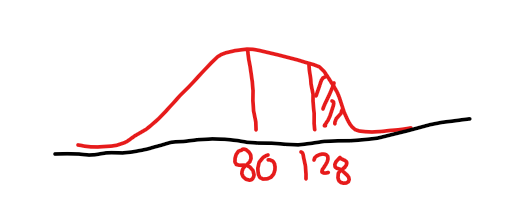
\includegraphics[scale=0.70]{mat2377_a1_img1.png}
        \newpage
        
        We need to find $P(W > 128)$, but we know that $W = rV^2$, so by substitution, we have,
        $$P(W > 128) = P(rV^2 > 128)$$
        Manipulating the equation, we have,
        $$P(rV^2 > 128) = P\left(V > \sqrt{\dfrac{128}{r}}\right) = P\left(V > \sqrt{\dfrac{128}{(2)}}\right) = P(V>8)$$
        Now, find the z-value.
        \begin{align*}
            z &= \dfrac{V-\mu}{\sigma}\\
            z &= \dfrac{V-E[V]}{SD[V]}\\
            z &= \dfrac{8-6}{2}\\
            z &= 1
        \end{align*}
        Since $z = 1.00$, referring to Table $A.3$, we have that the area under the curve that corresponds to the z-value of 1 is $0.8413$. Multiplying this value by 100\%, we have that
        $$P(V<8) = 84.13\%$$
        This gets us the area under the curve from 0 to 8, however, we want $P(V>8)$, not $P(V<8)$. So,
        \begin{align*}
            P(V<8) &= 84.13\%\\
            P(V>8) &= 100\% - 84.13\%\\
            P(V>8) &= 15.87\%
        \end{align*}
        Therefore, the probability of $P(W>128) = 15.87\%$.
    \end{enumerate}
    
    


\end{enumerate}






\end{document} 
